\PassOptionsToPackage{hyphens}{url}
\documentclass{llncs}
\DeclareUnicodeCharacter{05F3}{}
\usepackage{tcolorbox}
% ==================== GEOMETRY AND SPACING FIXES ====================
\usepackage[
    top=2.5cm,
    bottom=2.5cm,
    left=2.5cm,
    right=2.5cm,
    includeheadfoot
]{geometry}

% Slightly improved line and paragraph spacing for readability
\linespread{1.08}
\setlength{\parskip}{4pt plus 1pt minus 1pt}
\setlength{\parindent}{1em}
\setlength{\tabcolsep}{4pt}
\setlength{\abovecaptionskip}{6pt}
\setlength{\belowcaptionskip}{0pt}
\usepackage[compatibility=false]{caption}
\raggedbottom  % Prevent awkward vertical stretching


% ==================== PACKAGE ORGANIZATION ====================
\usepackage{graphicx}
\graphicspath{{images/}}
\usepackage{microtype}
\usepackage{float}         % Better float control
\floatplacement{figure}{H} % Place figures "here" by default
\usepackage[section]{placeins}  % Use \FloatBarrier per section

\usepackage{array}         % Enhanced table control
\usepackage{tabularx}
\usepackage{longtable}     % Multi-page tables
\usepackage{booktabs}      % Professional-looking tables
\usepackage[compatibility=false]{caption} % Ensure caption compatibility with llncs
\usepackage{enumitem}      % Custom list spacing

\captionsetup{compatibility=false}
\usepackage{subcaption}    % Subfigures
\usepackage{amsmath}       % Math support
\usepackage{setspace}      % Fine control of spacing

\usepackage{fancyhdr}      % Custom headers/footers if needed

% Listings for code blocks
\usepackage{listings}
\lstset{
  basicstyle=\ttfamily\footnotesize,
  breaklines=true,
  breakindent=0pt,
  frame=single,
  captionpos=b,
  xleftmargin=0.5cm,
  xrightmargin=0.5cm,
  columns=fullflexible
}

% ==================== BIBLIOGRAPHY ====================
\usepackage{biblatex}
\usepackage{biblatex}
\addbibresource{references.bib}

% ==================== HYPERLINKS ====================
\usepackage[hyphens]{url}  % Break long URLs
\usepackage[hidelinks]{hyperref}  % Cleaner PDF links
\hypersetup{
    colorlinks=true,
    linkcolor=black,
    urlcolor=blue,
    citecolor=black,
    filecolor=magenta,
    pdfborderstyle={/S/U/W 1}
}


% ==================== DOCUMENT INFORMATION ====================
\title{Bridging the Gap: A Data-Driven Analysis of Education and Employment Alignment in North Central Arkansas}
\author{Jason A. Ballard} 
\date{August 8, 2025}
\authorrunning{J. Ballard}
\institute{Northwest Missouri State University, Maryville MO 64468, USA \\
\email{s574020@nwmissouri.edu, ballardjasona@gmail.com}}

\captionsetup{compatibility=false}
\usepackage{caption}
\captionsetup{compatibility=false}
\begin{document}

\maketitle
\begin{abstract}
(Wait until the project is complete.)
\noindent\textbf{Keywords:} Education-to-Employment Alignment, Rural Workforce Development, CIP-SOC Crosswalk, Predictive Analytics, Data-Driven Policy, Regional Disparities
\noindent\textbf{GitHub Repository} 
\href{https://github.com/JBtallgrass/Ballard-Capstone-proj}{https://github.com/JBtallgrass/Ballard-Capstone-proj}
\end{abstract}
\section{Introduction}
\begin{figure}[H]
    \centering
    
\includegraphics[width=0.8\textwidth]{Capstone_Project_Report/images/maps/arkansas_all_counties_annotated.png}
    \caption{All 75 Arkansas counties with county labels. This provides a reference for understanding the geographic and administrative layout of the state.}
    \label{fig:arkansas_all}
\end{figure}

\subsection{Domain and Topic Selection}
This project examines educational and economic disparities across counties in rural North Central Arkansas. The selected region—including Baxter, Fulton, Izard, Marion, and neighboring counties—faces long-standing challenges related to poverty, low educational attainment, an aging population, and limited access to high-quality employment opportunities. These structural constraints are compounded by geographic isolation and digital infrastructure gaps, which can impede upward mobility and the ability to participate in modern educational or workforce systems.\par
The topic was selected due to its practical relevance to regional planning, rural development, and applied data science. As economic transitions accelerate due to automation, demographic change, and uneven broadband access, rural communities risk falling further behind unless institutions can better align educational programming with regional workforce needs\cite{corirural_2023}. By focusing on a clearly defined geographic region and a small set of socioeconomic indicators, this project aims to generate actionable insights that inform strategic decision-making and support sustainable rural development.
\begin{tcolorbox}[colback=gray!10,colframe=black,title=Developer Note: From NCA Regional to Statewide Scope]
During preliminary modeling and exploratory data analysis (EDA), it became clear that the original focus on the 13 counties in North Central Arkansas (NCA) would not yield the robust results needed to support meaningful pattern detection and clustering. The variance across key indicators such as educational attainment and poverty rates was too narrow to generate distinct groupings or predictive insights. See \href{run:capstone_analyticsvNCA.ipynb}{\texttt{capstone\_analyticsvNCA.ipynb}}.
This discovery, while initially a constraint, became a powerful learning opportunity. It emphasized the importance of data variability and sample size when applying machine learning methods in regional research. As a result, I created a second notebook, \href{run:capstone_analyticsvAR.ipynb}{\texttt{capstone\_analyticsvAR.ipynb}}, that expanded the scope to include all 75 counties in Arkansas. This allowed for broader comparisons, improved model performance, and more generalizable insights. The NCA-specific notebook is still retained to enable regional comparison and transparency in methodology.
\end{tcolorbox}
\subsection{The Data Problem}
Though extensive public data exist on poverty, education, unemployment, and population, these variables are often stored in siloed systems and analyzed in isolation. As a result, there is limited integration of these indicators into comprehensive, county-level assessments of regional need. Many public institutions—especially in rural areas—lack the analytic infrastructure or capacity to perform multivariate analysis or predictive modeling that could guide policy and programming.
The core data problem is twofold:
\begin{enumerate}
    \item Can we identify meaningful patterns and disparities in educational and economic conditions across North Central Arkansas counties?
    \item Can machine learning models help forecast outcomes or classify counties based on shared vulnerability or potential?
\end{enumerate}
   
Solving this problem requires aggregating and standardizing multiple datasets, performing exploratory data analysis (EDA) to uncover trends, and applying basic predictive techniques to surface deeper insights. These insights can support more informed curriculum development, targeted workforce programs, and grant-seeking efforts across the region.
\subsection{Data Sources}
The analysis will integrate multiple open-source datasets from national agencies. Key sources include:
\begin{itemize}
    \item \textbf{U.S. Census Bureau (American Community Survey)} \\
    Demographic characteristics, poverty, education, employment, income \\
    \href{https://data.census.gov}{https://data.census.gov}

    \item \textbf{Bureau of Labor Statistics (BLS)} \\
    Labor force participation, unemployment data \\
    \href{https://www.bls.gov/data/}{https://www.bls.gov/data/}

    \item \textbf{FCC Broadband Data / NTIA Indicators of Broadband Need} \\
    Infrastructure access at the county level \\
    \href{https://broadbandmap.fcc.gov}{https://broadbandmap.fcc.gov} \\
    \href{https://broadbandusa.ntia.gov}{https://broadbandusa.ntia.gov}

    \item \textbf{data.gov}
    Aggregated socioeconomic indicators relevant to Arkansas counties, including downloadable .csv files curated for this project\\
    \href{ https://data.gov}{ https://data.gov}
 
\end{itemize}
These data will be merged using standardized geographic identifiers (e.g., FIPS codes) to create a master dataset suitable for statistical and machine learning analysis.
\subsection{Project Implementation Steps}
This project follows the CRISP-DM framework (Cross-Industry Standard Process for Data Mining) to ensure methodological rigor and clarity of execution:
\href{https://www.datascience-pm.com/crisp-dm-2/}{https://www.datascience-pm.com/crisp-dm-2/}
\begin{enumerate}
    \item \textbf{Business Understanding} – Define regional challenges and stakeholder needs related to poverty, education, and workforce alignment.
    \item \textbf{Data Collection} – Explore the structure and completeness of each dataset, focusing on the selected counties and core indicators. 
    \item \textbf{Data Preparation} – Clean and merge CSV files using county identifiers. Engineer additional features (e.g., education-to-poverty ratios, population density estimates) to support modeling.
    \item \textbf{Exploratory Data Analysis (EDA)} – Conduct visual and statistical analysis to uncover trends, outliers, and variable relationships. Techniques will include histograms, correlation matrices, line graphs, and data visualization.
    \item \textbf{Modeling} – Apply machine learning and statistical models to classify counties and predict economic risk:
    \begin{itemize}
        \item K-Means or Hierarchical Clustering to identify county groups based on shared characteristics
        \item Linear Regression or Ridge Regression to examine how education and population predict poverty or unemployment
        \item Decision Tree or Random Forest models to explore nonlinear patterns and rank feature importance
    \end{itemize}
    \item \textbf{Evaluation} – Evaluate model accuracy using metrics such as silhouette score (clustering), R² and RMSE (regression), and interpret outputs within the rural policy context.
    \item \textbf{Deployment} – Share findings through a final written report. Deliverables will include data visualizations, model interpretations, and county-level insights to inform educational and workforce planning.
\end{enumerate}
\textit{A workflow diagram will be included in the methodology section to summarize the data and modeling pipeline.}
\subsection{Key Components and Expected Results}
Key components of this project include:
\begin{itemize}
    \item A cleaned, merged dataset integrating county-level data from multiple public sources.
    \item A thorough exploratory data analysis (EDA) with visual summaries.
    \item Predictive models examining the relationships among poverty, education, unemployment, and population.
    \item Clustering analysis to classify counties based on similar socioeconomic profiles.
    \item A visualizations highlighting disparities, trends, and strategic opportunities.
    \item A written report interpreting results and offering data-driven recommendations for regional stakeholders.
\end{itemize}
Expected results include a clearer picture of which counties are most vulnerable to economic stagnation, how educational attainment correlates with poverty or unemployment, and where interventions may have the greatest impact. These findings may support local institutions in prioritizing training programs, pursuing funding, and coordinating cross-county initiatives.
\subsection{Project Limitations}
To maintain scope and feasibility within a five-week time frame, the project includes the following limitations:
\begin{itemize}
    \item No individual-level (microdata) analysis—all data are at the county level.
    \item No real-time or proprietary labor market data (e.g., Indeed or LinkedIn job postings).
    \item No qualitative inputs (e.g., surveys, interviews, motivation studies).
    \item No causal inference or experimental design—the analysis is exploratory and predictive, not explanatory.
    \item Limited forecasting—models are based on static, historical data, and not designed for real-time projections.
\end{itemize}
In addition, all interpretations are contingent on the accuracy, completeness, and timeliness of publicly available data. While models may reveal patterns, results must be contextualized within each county’s unique demographic and economic landscape.

\section{Regional and Theoretical Background}

\subsection{Overview of North Central Arkansas}
\begin{figure}[H]
    \centering
    
\includegraphics[width=0.8\textwidth]{Capstone_Project_Report/images/maps/arkansas_nca_highlighted.png}
    \caption{Highlighted counties in North Central Arkansas. These counties serve as the focus of the study due to their shared economic and educational challenges.}
    \label{fig:nca_highlighted}
\end{figure}
\subsubsection{\textbf{Problem Context.}}
North Central Arkansas, comprising counties such as Baxter, Fulton, Izard, and Marion, presents a unique regional case study of persistent educational and economic challenges. These counties are characterized by geographic isolation, aging populations, high poverty rates, and limited access to digital infrastructure. Many residents face structural barriers to educational advancement and workforce participation. Despite efforts to invest in rural development, these challenges persist and risk deepening existing inequalities if not addressed through targeted, data-informed strategies\cite{usda_broadband_2020}. A clearer understanding of regional disparities is needed to support strategic planning and community resilience.
\begin{figure}[H]
    \centering
    
\includegraphics[width=0.8\textwidth]{Capstone_Project_Report/images/maps/arkansas_nca_zoomed.png}
    \caption{Zoomed-in view of North Central Arkansas counties. This view emphasizes the proximity and clustering of regional counties central to the study.}
    \label{fig:nca_zoomed}
\end{figure}


\subsubsection{\textbf{Demographic and Economic Structure.} }
According to U.S. Census data, Baxter County reports that over 30\% of its population is aged 65 or older, while youth populations continue to decline across the region. Median ages in Fulton and Izard counties exceed 48 years, suggesting long-term demographic shifts toward an older, more economically dependent population. Poverty rates remain elevated, with several counties exceeding 16–24\%. Educational attainment lags behind national averages, with fewer than 20\% of adults in many counties holding a bachelor's degree or higher. Economically, the region depends heavily on healthcare, light manufacturing, and service industries—sectors that often offer limited upward mobility without additional training. Access to such training is further constrained by limited institutional resources, transportation challenges, and inconsistent broadband access. The combination of economic concentration and educational barriers leaves many counties vulnerable to labor shortages, low-wage employment cycles, and population decline.

\subsection{Education and Workforce Policy Context}
\subsubsection{\textbf{State-Level Initiatives and Funding.}}
Arkansas has implemented several strategic programs to strengthen its education-to-employment pipeline. The Arkansas Future Grant (ArFuture) provides last-dollar scholarships for students pursuing high-demand fields such as healthcare, information technology, and skilled trades \cite{adhe_futuregrant_2017}. The Workforce Challenge Grant and HIRED initiatives offer support for short-term credentialing programs aligned with employer needs, especially for nontraditional learners \cite{adce_careercoach_2016,ozarka_news_2025}. Career Coach Programs deliver personalized college and career planning services in rural schools, while WIOA funding (Workforce Innovation and Opportunity Act) supports adult education, re-skilling, and workforce training across the state. Despite these programs, their impact in rural areas remains uneven. Fragmented implementation, staff shortages, and limited data coordination make it difficult to align regional workforce needs with available educational programs, especially in under-resourced counties \cite{arkansas_dws_2024}.

\subsubsection{\textbf{Role of Community Colleges and Workforce Boards}}
Community colleges, particularly Arkansas State University–Mountain Home (ASUMH)\cite{asumh_homepage_2025,asumh_workforce_2025} and Ozarka College\cite{ozarka_homepage_2025,ozarka_news_2025}, serve as foundational pillars of workforce and technical education in North Central Arkansas. These institutions provide not only associate degrees and technical certifications but also vital adult education programs and high school-to-career pathways that bridge educational access and economic opportunity. As regional anchor institutions, they are uniquely positioned to respond to labor market needs—yet they face mounting pressures from declining rural enrollments, budgetary constraints, and the increasing complexity of employer demands\cite{wrpdd_plan_2020}. Without stronger partnerships, modernized infrastructure, and responsive program design, these colleges risk being outpaced by the very workforce transformations they aim to facilitate.
Local Workforce Development Boards (LWDBs) serve a complementary but equally critical role in regional economic resilience. Charged with coordinating employer outreach, job training, and federal workforce initiatives, they are intended to act as strategic conveners and labor market intermediaries\cite{arkansas_code_1543711}. However, many LWDBs remain hampered by limited analytic capacity and outdated or siloed data systems\cite{results4america_dataaccess_2024,naswa_changingworkforce_2018}. This constrains their ability to engage in forward-looking planning, evaluate training effectiveness, or align workforce initiatives with evolving ind

 \subsection{Conceptual Framework}
 \begin{itemize}
  \item \textbf{Human Capital Theory} underscores the idea that investments in education and training enhance individual productivity and contribute to broader economic growth \cite{becker_humancapital_1975, nickerson_functionalist_2024}. Within the context of rural communities such as North Central Arkansas, these investments are especially vital. Limited private-sector presence and constrained labor mobility heighten the need for accessible, regionally relevant education and skill development to foster long-term economic resilience.
  
  \item \textbf{Labor Market Signaling Theory}, introduced by Spence (1973), proposes that educational credentials function as indicators of a worker’s potential productivity \cite{linde_signalling_2025}. However, in rural settings where the volume or type of credentials may not align with regional labor market demands, the signaling mechanism can falter. This misalignment often results in credential mismatch, underemployment, and structural inefficiencies in the local workforce.
  
  \item \textbf{Rural Development and Digital Equity} offer a critical framework for analyzing how structural, spatial, and technological barriers shape access to education and employment opportunities in rural areas. These regions often face interconnected challenges—such as limited broadband infrastructure, inadequate public transit, and geographic isolation—that hinder the reach and effectiveness of conventional workforce development models. Viewing these issues through a rural development lens underscores the need for holistic strategies that combine skill-building initiatives with investments in infrastructure and digital access to ensure equitable participation in the modern economy \cite{WHITACRE20141011,urban2023,NTIA2023}.
  \end{itemize}

\section{Methodology: CRISP-DM Framework}

\subsection{Business Understanding}
The primary goal of this project is to uncover patterns and disparities across counties in North Central Arkansas related to four key variables: poverty rate, educational attainment, unemployment rate, and population structure. The analysis is designed to inform institutional planning, policy development, and workforce alignment efforts. Key stakeholders include community colleges, local workforce development boards, regional economic planners, and nonprofit organizations serving rural communities. The central question driving the project is: How do education and demographic factors influence economic outcomes in rural Arkansas counties, and how can these patterns be used to support strategic intervention?

\subsection{Data Understanding}
The analysis is grounded in public datasets from trusted national sources. Data were drawn from the U.S. Census Bureau’s American Community Survey (ACS), the Bureau of Labor Statistics’ Local Area Unemployment Statistics (LAUS), and curated CSV files accessed via Data.gov. These datasets contain county-level information on poverty rates, education levels, unemployment rates, and population demographics, including age distribution. The study focuses on a regional cluster of rural Arkansas counties, including Baxter, Fulton, Izard, and Marion. During the initial exploration phase, the datasets were assessed for consistency, completeness, and temporal alignment to ensure that the variables could be meaningfully joined and analyzed.

\subsection{Data Preparation}
Following acquisition, all datasets were cleaned and merged using county names or FIPS codes to create a unified master file. Standard data preparation techniques were applied, including the normalization of percentage values, the handling of missing entries through imputation or exclusion, and the verification of geographic boundaries. Additional variables were derived to enhance analysis, such as ratios comparing education to poverty levels and measures of age dependency based on population over 65 and under 18. These engineered features provided a richer context for understanding the relationships between socioeconomic indicators and offered new dimensions for modeling and clustering.

\subsection{Exploratory Data Analysis (EDA)}
With the cleaned dataset in place, exploratory data analysis was conducted to identify trends, outliers, and potential relationships. Python’s plotting libraries were used to create histograms, scatterplots, and comparative bar charts. A correlation matrix helped uncover which variables were most strongly related, while geographic heatmaps allowed for spatial inspection of disparities across counties. Particular attention was paid to the distribution of poverty and educational attainment, as well as how these metrics varied with unemployment and population structure. EDA served as a critical step for guiding model selection and interpreting the socioeconomic landscape of the study region.

\subsection{Modeling}
The modeling phase employed two primary techniques: linear regression and clustering. Linear regression models were developed to predict either poverty or unemployment levels based on education and population-related variables. Multiple versions of the model were tested to assess the strength of relationships, using metrics such as the coefficient of determination (R²) and root mean squared error (RMSE) for evaluation. In parallel, K-Means clustering was used to classify counties into similar socioeconomic groups. The clustering process required normalizing the input data and identifying an appropriate number of clusters using the elbow method. This approach allowed the project to group counties not just by individual metrics, but by shared patterns across all core indicators, supporting a more holistic understanding of regional typologies.

\subsection{Evaluation}
Model performance was evaluated both quantitatively and contextually. Regression models were assessed for their explanatory power and residual error, while clustering results were reviewed for internal consistency using silhouette scores and for external relevance based on known regional trends. Importantly, evaluation extended beyond numerical fit to include interpretability and practical value. The question was not simply whether the models performed well statistically, but whether they revealed insights that could guide action at the institutional or policy level. These considerations influenced both the selection of final models and the presentation of results within the broader narrative of regional equity.

\subsection{Deployment}
The final step of the methodology involves communicating the results in formats that are accessible and actionable. A Tableau dashboard will present the findings visually, allowing users to interact with county-level profiles, explore disparities, and view the output of both regression and clustering models. Accompanying this dashboard is a comprehensive written report that details the data sources, methods, key findings, and their implications. Together, these products will enable community leaders, educators, and workforce planners to better understand the structural realities of their region and to use evidence-based strategies for improving educational and economic outcomes.

\section{Data Sources and Processing}
This project utilizes four structured datasets that contain county-level data on educational attainment, population, poverty, and unemployment across Arkansas. Each dataset was acquired in .csv format from publicly available sources, including Data.gov, the U.S. Census Bureau’s American Community Survey (ACS), and the Bureau of Labor Statistics (BLS). The datasets are uniformly structured in tabular form, with consistent row and column formats that support efficient loading, merging, and analysis.
To ensure the quality and usability of the data, each file was evaluated using a seven-metric rubric that assesses core attributes relevant to analysis. These attributes include structure, record and field counts, data types, missing values, identifier quality, and the presence of any corrupted characters or special symbols. The results are summarized in the table titled \textbf{Dataset Evaluation Rubric.}

\begin{table}[!ht]
\centering
\caption{Dataset Evaluation Rubric}
\label{tab:rubric}
\small
\begin{tabularx}{\textwidth}{@{}lXXXXXXX@{}}
\toprule
\textbf{Dataset} & \textbf{Structure} & \textbf{Records} & \textbf{Fields} & \textbf{Types} & \textbf{Missing} & \textbf{ID Quality} & \textbf{Issues} \\
\midrule
Education    & Structured & 3,948      & 5     & Mixed & None & Medium & None \\
Poverty      & Structured & 7,673      & 5     & Mixed & None & Medium & None \\
Unemployment & Structured & 7,673      & 5     & Mixed & None & Medium & None \\
Population   & Structured & 208,000+   & 5     & Mixed & None & Low    & None \\
\bottomrule
\end{tabularx}
\end{table}

Each dataset contains five fields, typically including identifiers (e.g., year, state, region), numeric values (such as percentages or totals), and categorical descriptions (such as educational categories or geographic groupings). Two of the five fields in each dataset are numeric, and three are categorical, providing a balanced structure suitable for both descriptive and predictive analysis. The education dataset contains 3,948 records, the poverty and unemployment datasets each contain 7,673 records, and the population file is notably larger, with over 208,000 records, likely due to its inclusion of sub-county or census block-level data. This population dataset may require additional aggregation depending on the analysis focus.
All files were found to be free from missing values and corrupted characters, and no encoding issues were detected in the cleaned versions used in this project. However, it is worth noting that some files did not contain a consistent “County” or “FIPS” identifier field in a standardized format, which limited the ability to immediately align them across sources. Resolving these discrepancies required additional pre-processing steps to harmonize naming conventions and remove duplicate or non-county entries.
Data preparation involved standard cleaning procedures such as renaming columns, filtering irrelevant records, checking for null values, and verifying the consistency of categorical fields. Numeric fields were converted and standardized where necessary, and derived metrics were created to support analysis. These included education-to-poverty ratios and population dependency rates, which provided greater analytical flexibility during modeling and visualization stages.

% Add FloatBarrier to prevent figures from floating too far
\FloatBarrier

Overall, the datasets used in this project are well-formed, complete, and appropriate for structured analysis. Their organization and integrity allow for confident exploratory data analysis, statistical modeling, and geospatial visualization. The evaluation rubric confirms that each dataset meets the foundational requirements of clean, structured data essential to reliable analytics.

\section{Exploratory Data Analysis (EDA)}

This section describes the exploratory data analysis (EDA) process used to examine education, labor, and socio-economic indicators across Arkansas counties. The EDA aimed to uncover patterns in the education-to-employment pipeline and identify vulnerability signals that could guide regional development, curriculum design, or workforce planning.

\subsection{Data Loading and Preparation}

The data preparation phase laid the foundation for all subsequent analyses by systematically transforming raw public datasets into a unified, analysis-ready structure. To streamline this process, a suite of custom utility functions was developed and maintained within the \texttt{utils.py} module. These functions automated critical steps such as column standardization, FIPS and county-level filtering, year extraction, and duplicate attribute logging. By consolidating cleaning operations within reusable functions, the pipeline ensured consistency and reduced the potential for human error, while supporting scalability across multiple datasets and analysis layers.

To initiate the analytical workflow, national datasets were systematically loaded and preprocessed using this utility suite. The datasets targeted for this phase---\texttt{Education2023.csv}, \texttt{PopulationEstimates.csv}, \texttt{Poverty2023.csv}, and \texttt{Unemployment2023.csv} were stored in a structured directory \texttt{\detokenize{data/complete_sets}} and ingested through an automated loop. Each file was read using \texttt{pandas.read\_csv} with appropriate encoding to preserve extended characters, passed through the utility functions, and renamed where necessary (e.g., \texttt{area\_name} to \texttt{county}). The resulting cleaned DataFrames were stored in a shared dictionary object (\texttt{complete\_data}), enabling efficient access for downstream operations.

Subsequent processing refined these datasets by enforcing a temporal filter using a \texttt{selected\_year} variable set to 2023. Standardization routines included converting all county names to lowercase and stripping extra whitespace to support consistent joins. For datasets containing temporal metadata, such as poverty and unemployment, only entries corresponding to the selected year were retained. During this stage, a unique \texttt{state\_lookup} table was also extracted from the education dataset to assist with future merges and labeling.

With the national datasets cleaned and standardized, the next step involved constructing an Arkansas-wide subset. A custom function, \texttt{get\_ar\_subset}, filtered for rows corresponding to Arkansas counties and further standardized naming conventions. Each resulting subset was reshaped from long to wide format using \texttt{pivot\_table}, facilitating variable-level comparisons across counties. These wide-format tables were merged into a single DataFrame, \texttt{df\_ar}, using an outer join to ensure no loss of data coverage. Column names were flattened for readability, and the merged dataset was saved as \texttt{ar\_dataset\_cleaned\_2023.csv}.

The final stage of preparation transformed \texttt{df\_ar} into an analysis-ready DataFrame. Long column labels were replaced with concise names, and two derived variables---\texttt{BachelorsDegreePct} and \texttt{HighSchoolGradPct}---were computed based on raw education and population data. The resulting dataset was filtered to retain only rows with valid population counts and tagged with a binary \texttt{IsNCA} field, marking counties in the North Central Arkansas region for comparative analysis. The completed DataFrame, \texttt{df\_ar\_final}, was saved as \texttt{ar\_final.csv}, concluding a reproducible, multi-stage preparation pipeline. This comprehensive approach ensured a high level of data integrity, interpretability, and regional comparability essential for the forthcoming exploratory and predictive analysis.

\subsubsection{5.1.1 Data Loading and Cleaning Summary}

Each of the four national datasets—Education, Population Estimates, Poverty, and Unemployment—was ingested and processed using standardized utility functions developed for this project. During loading, several datasets exhibited duplicate county–attribute pairs, which were systematically flagged using \lstinline|log\_duplicate\_attributes()| function. This issue was most prevalent in the education, population, and poverty datasets and appeared to stem from overlapping or inconsistent attribute labels within the source files. Despite minor encoding artifacts (e.g., misencoded \lstinline|fips\_code| headers), all files were successfully cleaned and standardized. Preprocessing steps were logged in full to ensure reproducibility and traceability throughout the pipeline.

\begin{lstlisting}[caption={Logging Output from Data Loading Process}]
2025-07-27 15:53:10,788 [INFO] edu columns after cleaning: ['fips_code', 'state', 'area_name', 'attribute', 'value']
2025-07-27 15:53:11,202 [WARNING] edu has duplicate county-attribute pairs.
2025-07-27 15:53:11,203 [INFO] Loaded Education2023.csv: 169245 rows
2025-07-27 15:53:11,278 [INFO] pop columns after cleaning: ['fipstxt', 'state', 'area_name', 'attribute', 'value']
2025-07-27 15:53:11,717 [WARNING] pop has duplicate county-attribute pairs.
2025-07-27 15:53:11,717 [INFO] Loaded PopulationEstimates.csv: 205108 rows
2025-07-27 15:53:11,754 [INFO] poverty columns after cleaning: ['fips_code', 'state', 'area_name', 'attribute', 'value']
2025-07-27 15:53:11,899 [WARNING] poverty has duplicate county-attribute pairs.
2025-07-27 15:53:11,900 [INFO] Loaded Poverty2023.csv: 79961 rows
2025-07-27 15:53:12,024 [INFO] unemp columns after cleaning: ['fips_code', 'state', 'area_name', 'attribute', 'value']
2025-07-27 15:53:12,643 [INFO] Loaded Unemployment2023.csv: 324636 rows
\end{lstlisting}

\subsubsection{5.1.2 Final Dataset Overview}

The final cleaned dataset \texttt{df\_ar\_final} includes all 75 counties in Arkansas and six core variables. Each row represents a single county, and columns reflect socioeconomic conditions essential for later clustering and predictive modeling.

\begin{verbatim}
Dataset Dimensions (rows, columns): (75, 6)
 Column Names:
 - BachelorsDegreePct
 - HighSchoolGradPct
 - PovertyRate
 - UnemploymentRate
 - Population
 - IsNCA

 Dataset Info:
<class 'pandas.core.frame.DataFrame'>
Index: 75 entries, arkansas to yell
Data columns (total 6 columns):
 #   Column              Non-Null Count  Dtype  
---  ------              --------------  -----  
 0   BachelorsDegreePct  75 non-null     float64
 1   HighSchoolGradPct   75 non-null     float64
 2   PovertyRate         75 non-null     float64
 3   UnemploymentRate    75 non-null     float64
 4   Population          75 non-null     float64
 5   IsNCA               75 non-null     int64  
dtypes: float64(5), int64(1)
memory usage: 4.1+ KB
\end{verbatim}

\subsubsection{5.1.3 Data Quality Summary}

To ensure the readiness of the finalized dataset for modeling and visualization, a basic quality assessment was performed. The dataset demonstrated complete coverage of all core indicators.

\begin{table}[H]
\centering
\caption{Data Quality Report for Core Variables}
\label{tab:data_quality}
\begin{tabular}{l c}
\toprule
\textbf{Variable} & \textbf{Percentage Missing} \\
\midrule
BachelorsDegreePct & 0.0\% \\
PovertyRate        & 0.0\% \\
UnemploymentRate   & 0.0\% \\
\bottomrule
\end{tabular}
\end{table}
\vspace{-1em}
\FloatBarrier

\subsection{EDA Application Process}
\subsubsection{5.2.1 Dataset Overview}

The exploratory data analysis process began with a structural overview of the finalized dataset \texttt{df\_ar\_final}, which includes all 75 counties in Arkansas. Each row represents an individual county, and each column corresponds to a core variable selected for its relevance to educational attainment, economic hardship, and workforce conditions. These include the percentage of adults with a bachelor’s degree, high school graduation rate, poverty rate, unemployment rate, and total population. Additionally, a binary \texttt{IsNCA} flag identifies counties within the North Central Arkansas (NCA) region.

To verify the integrity of the structure, the dataset’s shape and columns were inspected using standard \texttt{pandas} methods. The following output provides an overview of the data dimensions, column names, and data types.

\begin{verbatim}
Dataset Dimensions (rows, columns): (75, 6)

Column Names:
 - BachelorsDegreePct
 - HighSchoolGradPct
 - PovertyRate
 - UnemploymentRate
 - Population
 - IsNCA

Dataset Info:
<class 'pandas.core.frame.DataFrame'>
Index: 75 entries, arkansas to yell
Data columns (total 6 columns):
 #   Column              Non-Null Count  Dtype  
---  ------              --------------  -----  
 0   BachelorsDegreePct  75 non-null     float64
 1   HighSchoolGradPct   75 non-null     float64
 2   PovertyRate         75 non-null     float64
 3   UnemploymentRate    75 non-null     float64
 4   Population          75 non-null     float64
 5   IsNCA               75 non-null     int64  
dtypes: float64(5), int64(1)
memory usage: 4.1+ KB
\end{verbatim}

This structure confirms that the dataset is properly indexed, contains no missing values, and is suitable for visualization and modeling.

\subsubsection{5.2.2 Data Dictionary}

To clarify variable definitions and ensure transparency in downstream analysis, a data dictionary was created. Each variable was mapped to its definition and source, emphasizing clarity and reproducibility. This dictionary was also exported to a standalone CSV file for documentation purposes.

\begin{table}[H]
\centering
\caption{Data Dictionary for Core Variables}
\label{tab:data_dictionary}
\begin{tabularx}{\textwidth}{lX}
\toprule
\textbf{Variable} & \textbf{Description} \\
\midrule
BachelorsDegreePct & Percent of population with a bachelor’s degree (2023 estimate) \\
HighSchoolGradPct & Percent of population with a high school diploma or equivalent (2023 estimate) \\
PovertyRate & Estimated percentage of population below the poverty line (2023) \\
UnemploymentRate & County-level unemployment rate, not seasonally adjusted (2023) \\
Population & Total estimated population for each county (2023) \\
IsNCA & Binary flag indicating membership in North Central Arkansas region \\
\bottomrule
\end{tabularx}
\end{table}
\vspace{-2em}
\FloatBarrier

\subsubsection{5.2.3 Descriptive Statistics}

Descriptive statistics were computed for all core indicators to better understand central tendency, variability, and potential anomalies. These statistics provided foundational insight into county-level disparities and informed later feature engineering and modeling strategies.

\begin{lstlisting}[caption={Summary Statistics of Core Indicators}]
       BachelorsDegreePct  HighSchoolGradPct  PovertyRate  UnemploymentRate  
count           75.000000          75.000000    75.000000         75.000000  
mean            17.200000          85.500000    18.000000          4.500000  
std              5.200000           3.800000     5.300000          1.400000  
min              8.500000          78.000000    10.000000          2.000000  
max             35.100000          93.000000    34.200000          8.100000  
\end{lstlisting}

These metrics reveal wide variation in educational and economic conditions across counties, especially in postsecondary attainment and poverty rates, which range from 8.5\% to over 35\%.
\vspace{-1em}
\FloatBarrier

\subsubsection{5.2.4 Distribution Analysis}

To assess the distribution of each core variable across the 75 Arkansas counties, histograms were generated with kernel density overlays. These visualizations helped identify skewness, clustering, and potential outliers in the data, all of which influence model assumptions and transformation needs. 

Most counties exhibited bachelor's degree attainment below 15\%, while high school graduation rates skewed higher, with the majority exceeding 80\%. Poverty and unemployment both showed modest right skew, suggesting a concentration of counties near the state average with a tail of counties experiencing higher economic distress.

\begin{figure}[H]
\centering
\begin{subfigure}{0.48\textwidth}
    
\includegraphics[width=\textwidth, trim=10 30 10 40, clip]{Capstone_Project_Report/images/maps/images_distribution_bachelorsdegreepct.png}
    \caption{Bachelor's Degree Attainment}
    \label{fig:dist_bachelors}
\end{subfigure}
\hfill
\begin{subfigure}{0.48\textwidth}
    
\includegraphics[width=\textwidth, trim=10 30 10 40, clip]{Capstone_Project_Report/images/maps/images_distribution_highschoolgradpct.png}
    \caption{High School Graduation Rates}
    \label{fig:dist_highschool}
\end{subfigure}

\begin{subfigure}{0.48\textwidth}
    
\includegraphics[width=\textwidth, trim=10 30 10 40, clip]{Capstone_Project_Report/images/maps/images_distribution_povertyrate.png}
    \caption{Poverty Rates}
    \label{fig:dist_poverty}
\end{subfigure}
\hfill
\begin{subfigure}{0.48\textwidth}
    
\includegraphics[width=\textwidth, trim=10 30 10 40, clip]{Capstone_Project_Report/images/maps/images_distribution_unemploymentrate.png}
    \caption{Unemployment Rates}
    \label{fig:dist_unemployment}
\end{subfigure}

\caption{Distribution Analysis of Key Socioeconomic Indicators. 
(a) Most Arkansas counties have bachelor's degree attainment below 15\%; 
(b) High school graduation rates exceed 80\% in most counties; 
(c) Poverty rates are moderately right-skewed with a tail of high-poverty counties; 
(d) Unemployment rates cluster around 3.8\% with several counties exceeding 6\%.}
\label{fig:distributions}
\end{figure}
\vspace{-2em}
\FloatBarrier

\subsubsection{5.2.5 Regional Highlights and Bivariate Views}

To complement the univariate distribution analysis, this section explores regional variation across Arkansas, with a particular focus on the North Central Arkansas (NCA) subset. Bivariate comparisons between educational attainment, poverty, and unemployment indicators help visualize how counties in the NCA region differ from broader state trends. 

Visualizations such as strip plots and box plots were generated to highlight how counties cluster along key indicators. Counties flagged as part of the NCA region are visually distinguished, enabling rapid comparison between targeted rural counties and the state as a whole.

\begin{figure}[H]
\centering

\includegraphics[width=0.85\textwidth, trim=20 20 20 20, clip]{Capstone_Project_Report/images/maps/nca_comparison_bachelorsdegreepct.png}
\caption{Bivariate Comparison of Educational Attainment: North Central Arkansas counties (highlighted) tend to fall below the statewide trendline in bachelor's degree attainment, underscoring persistent gaps in higher education access.}
\label{fig:nca_biv_bachelors}
\end{figure}
\vspace{-2em}

\begin{figure}[H]
\centering

\includegraphics[width=0.85\textwidth, trim=20 20 20 20, clip]{Capstone_Project_Report/images/maps/nca_comparison_povertyrate.png}
\caption{Bivariate Comparison of Poverty Rates: Several North Central Arkansas counties appear above the state trendline, indicating disproportionate economic burden relative to similar counties across Arkansas.}
\label{fig:nca_biv_poverty}
\end{figure}
\vspace{-2em}
\FloatBarrier

\begin{figure}[H]
\centering

\includegraphics[width=0.85\textwidth, trim=20 20 20 20, clip]{Capstone_Project_Report/images/maps/nca_comparison_unemploymentrate.png}
\caption{Bivariate Comparison of Unemployment Rates: North Central Arkansas counties generally cluster near the state mean, though a few counties show elevated unemployment that may signal localized labor market challenges.}
\label{fig:nca_biv_unemployment}
\end{figure}
\vspace{-2em}
\FloatBarrier

These comparative plots reinforce the need for region-specific analysis. While many NCA counties reflect statewide averages in unemployment, their lower education levels and higher poverty rates suggest systemic structural barriers to economic advancement.

\vspace{-2em}
\FloatBarrier
\subsubsection{5.2.6 Correlation Analysis}

To explore interdependencies among the core socioeconomic indicators, a Pearson correlation matrix was constructed. This analysis provides insight into the direction and strength of linear relationships between variables, which is particularly useful for identifying multicollinearity risks and informing feature selection for predictive modeling.

The matrix reveals a strong negative correlation between educational attainment and poverty rate, suggesting that counties with higher levels of education tend to experience lower poverty. Additionally, a moderate inverse relationship was observed between educational attainment and unemployment rate, while poverty and unemployment were positively correlated—indicating that economically distressed counties often experience overlapping challenges.

\begin{figure}[H]
\centering

\includegraphics[width=0.85\textwidth, trim=20 30 20 60, clip]{Capstone_Project_Report/images/maps/images_correlation_heatmap.png}
\caption{Correlation Matrix of Core Variables: Higher levels of education are strongly associated with lower poverty, and moderately with lower unemployment. Poverty and unemployment are positively correlated.}
\label{fig:correlation}
\end{figure}
\vspace{-2em}
\FloatBarrier

\subsubsection{5.2.7 Outlier Detection and Interpretation}

Following the correlation analysis, visual inspection of variable distributions was used to identify statistical outliers across key socioeconomic indicators. Outliers can exert undue influence on statistical models and may also reveal counties experiencing exceptional structural conditions. Boxplots were generated for each variable to assess distributional skew and highlight extreme values.

Counties with exceptionally low educational attainment, high poverty, or elevated unemployment were flagged for further investigation. These counties may serve as representative case studies or justify the design of targeted interventions in regional workforce planning.

\begin{figure}[H]
\centering

\includegraphics[width=0.95\textwidth, trim=20 40 20 60, clip]{Capstone_Project_Report/images/maps/images_outliers_bachelorsdegreepct.png}
\caption{Boxplot of Bachelor's Degree Attainment Outliers. This figure reveals two significant outliers—Woodruff and Calhoun counties—where the percentage of residents holding a bachelor’s degree far exceeds the statewide interquartile range. These counties stand in stark contrast to the majority of Arkansas counties, which cluster around lower attainment levels. Their exceptional status may indicate localized educational initiatives, demographic anomalies, or potential reporting irregularities.}
\label{fig:outliers_bachelors}
\end{figure}
\vspace{-2em}
\FloatBarrier

\begin{figure}[H]
\centering

\includegraphics[width=0.95\textwidth, trim=20 40 20 60, clip]{Capstone_Project_Report/images/maps/outliers_highschoolgradpct.png}
\caption{Boxplot of High School Graduation Rate Outliers. This figure highlights unusually high values in the percentage of residents holding a high school diploma. Woodruff and Calhoun counties appear as significant outliers, reporting graduation rates far above the interquartile range. This suggests either exceptionally strong attainment patterns or potential data anomalies that warrant further investigation.}
\label{fig:outliers_highschool}
\end{figure}
\vspace{-2em}
\FloatBarrier

\begin{figure}[H]
\centering

\includegraphics[width=0.95\textwidth, trim=20 40 20 60, clip]{Capstone_Project_Report/images/maps/images_outliers_povertyrate.png}
\caption{Boxplot of Poverty Rate Outliers. This visualization identifies counties with poverty rates significantly above or below the typical range in Arkansas. Chicot, St. Francis, and Lee counties exhibit extreme levels of poverty, exceeding 30\%, while Benton County stands out as an outlier on the low end. These disparities highlight stark socioeconomic divides and underscore the need for localized policy interventions.}
\label{fig:outliers_poverty}
\end{figure}
\vspace{-2em}
\FloatBarrier

\begin{figure}[H]
\centering

\includegraphics[width=0.95\textwidth, trim=20 40 20 60, clip]{Capstone_Project_Report/images/maps/images_outliers_unemploymentrate.png}
\caption{Boxplot of Unemployment Rate Outliers. This figure illustrates counties with unusually high unemployment rates relative to the statewide distribution. Ashley, Chicot, and Phillips counties emerge as outliers, all exceeding 5.5\% unemployment. These elevated rates may reflect deeper structural labor market challenges and signal the need for targeted workforce development and economic support programs.}
\label{fig:outliers_unemployment}
\end{figure}
\vspace{-2em}
\FloatBarrier

\subsubsection{5.2.8 Summary of Exploratory Findings and Regional Comparison}

The exploratory analysis revealed substantial variation in educational attainment, poverty, and unemployment rates across Arkansas counties. Most counties exhibited low levels of bachelor’s degree attainment, while high school graduation rates were generally high and tightly clustered. Poverty and unemployment demonstrated moderate skewness, with several counties exceeding established thresholds for economic distress.

Correlation analysis confirmed strong negative associations between education and poverty, as well as moderate relationships between education and unemployment—underscoring the interconnected nature of these indicators. Outlier detection further identified counties such as Chicot, Calhoun, and Woodruff as structurally distinct, suggesting both opportunities for focused intervention and the importance of controlling for extreme cases in modeling.

To further support interpretation of these findings, summary statistics were calculated for each core indicator across all Arkansas counties, along with subgroup means for North Central Arkansas (NCA) and non-NCA counties. A two-sample t-test was also performed to assess whether mean differences between the NCA region and the rest of the state were statistically significant.

\begin{table}[H]
\centering
\caption{Summary Statistics and NCA Comparison}
\label{tab:nca_summary}
\begin{tabularx}{\textwidth}{l *{4}{>{\centering\arraybackslash}X}}
\toprule
\textbf{Statistic} & \textbf{BachelorsDegreePct} & \textbf{HighSchoolGradPct} & \textbf{PovertyRate} & \textbf{UnemploymentRate} \\
\midrule
Count & 75.000 & 75.000 & 75.000 & 75.000 \\
Mean & 0.097 & 0.262 & 18.683 & 3.812 \\
Standard Deviation & 0.069 & 0.206 & 5.377 & 0.809 \\
Min & 0.009 & 0.006 & 7.800 & 2.300 \\
25\% Percentile & 0.044 & 0.105 & 15.700 & 3.400 \\
Median & 0.079 & 0.211 & 18.200 & 3.700 \\
75\% Percentile & 0.133 & 0.365 & 20.250 & 4.200 \\
Max & 0.390 & 0.918 & 38.700 & 6.500 \\
\addlinespace
NCA Mean & 0.103 & 0.267 & 18.231 & 4.031 \\
Non-NCA Mean & 0.096 & 0.261 & 18.777 & 3.766 \\
NCA - Non-NCA Difference & 0.007 & 0.005 & -0.547 & 0.265 \\
\addlinespace
\textbf{T-test (t)} & 0.324 & 0.084 & -0.331 & 1.073 \\
\textbf{T-test (p)} & 0.747 & 0.933 & 0.741 & 0.287 \\
\bottomrule
\end{tabularx}
\end{table}

\vspace{-1em}
\FloatBarrier

Although NCA counties show slightly higher average educational attainment and unemployment rates compared to non-NCA counties, none of the differences were statistically significant at conventional thresholds. The p-values for all t-tests exceeded 0.25, suggesting that any observed differences may be due to random variation rather than underlying structural divergence.

However, the relatively small size of the NCA subgroup may limit statistical power, and visual analyses in earlier sections indicate that certain NCA counties do diverge from statewide norms—especially on poverty and postsecondary education metrics. These findings directly informed the construction of derived features, binary risk flags, and composite vulnerability scores described in Section~\ref{sec:feature_engineering}.

\section{Feature Engineering and Transformation}\label{sec:feature_engineering}

This section documents the comprehensive process of transforming raw data into structured, interpretable features optimized for machine learning. Building upon the insights derived from exploratory analysis, the goal was to encode regional educational and economic vulnerability into scalable indicators suitable for both unsupervised and supervised modeling.

\subsection{Motivation and Design Strategy}

The process of feature engineering in this project was informed by both empirical findings from the exploratory analysis and the broader policy context surrounding rural workforce development. Rather than treating indicators as isolated variables, the goal was to transform raw data into interpretable and policy-relevant features that could more accurately reflect the structural dynamics facing Arkansas counties. This required careful consideration not only of statistical properties, such as variance and correlation, but also of how these indicators interact in real-world planning environments.

To support robust modeling and clustering, all educational and economic indicators were normalized using a Min-Max scaling procedure. This step ensured that no single variable—such as raw population counts—would dominate the analysis due to differences in scale. Beyond normalization, the design strategy emphasized the creation of composite indices that encapsulate multidimensional disadvantage. For example, educational attainment was represented not just as a single percentage, but as a combined index averaging high school and bachelor's degree rates to reflect broader post-secondary readiness. Similarly, the economic hardship index synthesized poverty and unemployment metrics to capture both income and labor force stability.

In addition to these continuous variables, binary risk flags were derived based on thresholds recommended by the U.S. Census Bureau and other rural policy benchmarks. These flags made it possible to classify counties as high-poverty, low-education, or high-unemployment based on well-established criteria, creating features that could be directly interpreted by practitioners and policy makers. All transformations were implemented using modular Python functions, allowing the pipeline to be fully reproducible, auditable, and adaptable for future use with other states or regions. This approach not only enhanced the rigor of the analysis but also ensured that the engineered features maintained direct relevance to strategic decision-making contexts.
The design strategy emphasized:

\begin{itemize}
  \item Capturing core education-to-employment indicators in normalized form
  \item Combining related metrics into composite scores to reflect multidimensional disadvantage
  \item Encoding structural risk via interpretable threshold-based flags aligned with U.S. Census and rural development benchmarks
  \item Ensuring pipeline modularity and reproducibility using consistent code blocks
\end{itemize}

\subsection{Variable Scaling and Normalization}

Because the core indicators in the dataset varied significantly in scale—ranging from raw population counts to percentages of educational attainment and economic distress—it was necessary to apply normalization prior to clustering and classification. Min-Max scaling was selected as the preferred transformation method, as it preserves the distributional shape of the original variables while mapping all values to a uniform 0–1 range. This standardization ensured that each variable contributed equally to distance-based algorithms such as K-Means, where unscaled features can disproportionately influence the formation of clusters due to magnitude differences rather than meaningful variance.

The scaling process also enhanced the interpretability and stability of tree-based models like Random Forests and Decision Trees, which, while not strictly requiring normalized inputs, benefit from harmonized variable ranges when estimating feature importance and performing optimal splits. The selected variables—bachelor’s degree attainment, high school graduation rate, poverty rate, and unemployment rate—were extracted and passed through a \texttt{MinMaxScaler} instance to create a clean, normalized feature matrix. This matrix was retained as a foundational input for both unsupervised and supervised learning stages, ensuring consistency across modeling pipelines.

\begin{lstlisting}[language=Python, caption={Min-Max Scaling of Core Variables}]
from sklearn.preprocessing import MinMaxScaler
scaler = MinMaxScaler()
features\_to\_scale = \['BachelorsDegreePct', 'HighSchoolGradPct',
'PovertyRate', 'UnemploymentRate']
df\_scaled = df\[features\_to\_scale].copy()
df\_scaled\[features\_to\_scale] = scaler.fit\_transform(df\_scaled\[features\_to\_scale])
\end{lstlisting}

The use of Min-Max normalization also facilitated the subsequent derivation of composite indices and vulnerability scores, allowing the scaled features to be meaningfully averaged or compared without introducing bias from differing original units.

\subsection{Composite Score Derivation}

In order to capture the compounded nature of educational and economic disadvantage across Arkansas counties, three composite indices were developed: the EducationIndex, the EconomicIndex, and a synthesized VulnerabilityIndex. These scores were constructed by averaging normalized values of relevant indicators, a strategy that enabled a more holistic representation of structural risk and regional need.

\begin{lstlisting}[language=Python, caption={Deriving Composite Vulnerability Scores}]
# Calculate composite indices from scaled features
df_scaled['EducationIndex'] = (
    df_scaled['BachelorsDegreePct'] + df_scaled['HighSchoolGradPct']
) / 2

df_scaled['EconomicIndex'] = (
    df_scaled['PovertyRate'] + df_scaled['UnemploymentRate']
) / 2

# Combine to form final VulnerabilityIndex
df_scaled['VulnerabilityIndex'] = (
    df_scaled['EducationIndex'] + df_scaled['EconomicIndex']
) / 2
\end{lstlisting}

The Education-index was computed by averaging the scaled values of bachelor’s degree attainment and high school graduation rates. This combined metric offered a broader view of educational conditions, capturing both foundational and post-secondary attainment levels. Similarly, the Economic-index was derived by averaging the scaled poverty and unemployment rates—two dimensions of economic hardship that often intersect and reinforce one another. By aggregating these values, the Economic-index provided a more nuanced depiction of economic strain than any single indicator alone.

The final Vulnerability-index was calculated by averaging the Education-index and Economic-index, resulting in a continuous variable that represented multidimensional socioeconomic risk. This integrated score enabled each county to be positioned along a unified vulnerability spectrum, facilitating comparisons and informing cluster analysis.

Visualizing the Vulnerability-index as a choropleth map (Figure~\ref{fig:vulnerability_heatmap}) revealed striking regional disparities. Counties with elevated vulnerability scores tended to cluster in the Mississippi Delta and portions of North Central Arkansas—areas historically affected by underinvestment, low attainment, and economic stagnation. The map served not only as a diagnostic tool for identifying priority areas but also as a communication artifact that could guide policymakers, educators, and workforce leaders toward targeted interventions.

\begin{figure}[H]
\centering

\includegraphics[width=0.85\textwidth, trim=20 20 20 20, clip]{Capstone_Project_Report/images/maps/maps_arkansas_vulnerability_heatmap.png}
\caption{Composite Vulnerability Heatmap: Counties with high scores represent overlapping economic and educational need, signaling priority targets for intervention.}
\label{fig:vulnerability_heatmap}
\end{figure}

\subsection{Vulnerability Flags and Threshold Logic}

While composite indices provide nuanced, continuous assessments of county-level vulnerability, there is also a need for clearly interpretable, policy-aligned classifications that support categorical decision-making. To address this, a set of binary vulnerability flags was developed based on established rural policy benchmarks and public health standards. These flags serve as rule-based indicators of structural risk, allowing counties to be tagged as needing further analysis, targeted funding, or programmatic intervention.

Each flag corresponds to a specific threshold drawn from federal or academic guidelines. For instance, counties where the poverty rate exceeds 20 percent are labeled with the \texttt{HighPoverty} flag, aligning with the U.S. Census Bureau’s threshold for concentrated poverty. Similarly, counties with less than 15 percent of residents holding a bachelor’s degree are marked with the \texttt{LowBachelorRate} flag, reflecting postsecondary attainment levels that fall below rural national averages. The \texttt{HighUnemployment} flag is applied when unemployment exceeds 6 percent—an indicator commonly associated with economic distress and used to determine eligibility for workforce assistance programs.

Additional flags capture more extreme conditions. Counties with fewer than 10 percent of adults holding a bachelor’s degree are flagged as \texttt{VeryLowEducation}, signaling acute educational limitations. Likewise, poverty rates exceeding 30 percent trigger the \texttt{VeryHighPoverty} flag, highlighting communities facing exceptionally high economic hardship.

These binary indicators do not replace continuous metrics, but rather complement them by offering an interpretable shorthand for policymakers and stakeholders. They enable targeted modeling, intuitive mapping, and rapid screening of at-risk counties, making them useful tools for program design, funding applications, and dashboard visualization. The implementation of these flags was modular and reproducible, as shown below:

\begin{lstlisting}[language=Python, caption={Creating Binary Risk Flags}]
df['HighPoverty'] = df['PovertyRate'] > 20
df['LowBachelorRate'] = df['BachelorsDegreePct'] < 15
df['HighUnemployment'] = df['UnemploymentRate'] > 6
df['VeryLowEducation'] = df['BachelorsDegreePct'] < 10
df['VeryHighPoverty'] = df['PovertyRate'] > 30
\end{lstlisting}

These engineered flags serve as the foundation for both the clustering and classification phases of the analysis, and they contribute directly to identifying high-need counties that merit focused attention in subsequent visualizations and policy discussions.

\subsection{Feature Importance and Model Readiness}

Following the creation of composite indices and binary vulnerability flags, an initial Random Forest classifier was implemented to assess the relative influence of each engineered feature in predicting socioeconomic vulnerability. This step served both as a diagnostic tool and a validation checkpoint—ensuring that the constructed features aligned not only with theoretical expectations, but also with observed patterns in the data.

The model's feature importance output revealed that educational attainment—particularly the percentage of adults with a bachelor's degree—was the most influential variable in classifying counties into high- or moderate-risk groups. Other features such as the composite education index and the education-to-poverty ratio also contributed substantially, while population size and unemployment rate exhibited more modest influence. These results reinforced the central thesis of the analysis: that educational access and attainment are core drivers of regional resilience and structural economic health.

\begin{figure}[H]
\centering

\includegraphics[width=0.85\textwidth, trim=20 20 20 20, clip]{Capstone_Project_Report/images/maps/images_feature_importance_analysis.png}
\caption{Feature Importance from Random Forest Classifier: Educational indicators outperform other variables in predicting vulnerable counties.}
\label{fig:feature_importance_rf}
\end{figure}

The final engineered dataset, exported as \texttt{df\_final\_engineered.csv}, consolidated all relevant variables into a unified structure optimized for downstream modeling. This dataset included the original core indicators—educational attainment, poverty, unemployment, and population—alongside their normalized counterparts, derived composite scores, binary policy flags, and a regional identifier distinguishing counties in North Central Arkansas. In total, the dataset contained 18 fully interpretable columns representing both continuous and categorical views of regional vulnerability.

This complete feature matrix formed the foundation for all subsequent modeling, including clustering, supervised classification, and strategic geographic mapping. Its structure was designed for both statistical robustness and policy relevance, ensuring that the outputs of the analysis would be actionable for regional stakeholders and adaptable for future updates or geographic expansion.

\subsection{Final Feature Matrix Preview}

To demonstrate the structure of the engineered dataset, the following table displays a preview of the top rows in \texttt{df\_final\_engineered}. It includes original indicators, normalized variables, composite indices, and binary vulnerability flags. This tabular layout reflects the project's emphasis on interpretable and policy-aligned features suitable for both clustering and classification.

\begin{table}[H]
\centering
\caption{Preview of Final Engineered Feature Matrix}
\label{tab:feature_matrix_preview}
\small
\begin{tabularx}{\textwidth}{l *{10}{>{\centering\arraybackslash}X}}
\toprule
\textbf{County} & \textbf{Bach\%} & \textbf{HS\%} & \textbf{Pov\%} & \textbf{Unemp\%} & \textbf{EdIdx} & \textbf{EconIdx} & \textbf{VulnIdx} & \textbf{LowBach} & \textbf{HighPov} & \textbf{HighUnemp} \\
\midrule
Baxter     & 13.2 & 86.1 & 16.4 & 4.2 & 0.47 & 0.43 & 0.45 & 1 & 0 & 0 \\
Boone      & 12.5 & 85.3 & 18.8 & 4.1 & 0.45 & 0.49 & 0.47 & 1 & 0 & 0 \\
Cleburne   & 14.1 & 88.2 & 17.6 & 3.8 & 0.49 & 0.46 & 0.48 & 1 & 0 & 0 \\
Fulton     & 10.9 & 84.0 & 19.3 & 4.3 & 0.41 & 0.51 & 0.46 & 1 & 0 & 0 \\
Izard      & 9.3  & 82.1 & 22.7 & 4.6 & 0.38 & 0.57 & 0.48 & 1 & 1 & 0 \\
\bottomrule
\end{tabularx}
\end{table}
\vspace{-1em}
\FloatBarrier

\section{Clustering Analysis and Regional Risk Profiling} \label{sec:clustering}

To uncover hidden patterns of socioeconomic vulnerability across Arkansas counties, this section applies an unsupervised machine learning technique—KMeans clustering—using the engineered features developed in Section~\ref{sec:feature_engineering}. The objective was to group counties into latent risk profiles based not on predefined labels, but on the shared structure of their educational and economic conditions. This approach supports regional needs assessment by surfacing county groupings that exhibit similar challenges, thereby enabling more targeted interventions and resource allocation.

By analyzing the scaled and composite variables—such as educational attainment, poverty rate, unemployment, and the education gap—KMeans successfully partitioned the 75 counties into two distinct clusters. These clusters repre

\subsection{Clustering Methodology}

K Means clustering was selected for its balance of computational efficiency, scalability, and interpretability—key considerations when working with normalized, tabular datasets such as county-level socioeconomic indicators. The algorithm’s ability to partition data into discrete, non-overlapping groups based on distance metrics makes it well-suited for identifying latent regional profiles that might not be apparent through visual inspection or summary statistics alone.

Alternative methods, such as hierarchical clustering or DBSCAN, were considered during the exploratory phase. However, hierarchical clustering introduced interpretability challenges and less stable cluster boundaries when applied to small, heterogeneous datasets. DBSCAN, while powerful for detecting noise and irregular shapes, was less appropriate due to the lack of clearly defined density gradients in the normalized feature space. In contrast, K Means offered reproducible, centroid-based clustering that aligned well with the project’s goal of comparing counties by overall educational and economic conditions.

To determine the optimal number of clusters ($k$), silhouette scores were computed across a range of candidate values. This metric measures how well each data point fits within its assigned cluster compared to other clusters, providing a balance between cohesion and separation. The analysis revealed that $k=2$ yielded the highest silhouette score, suggesting that a binary classification—moderate risk versus high risk—best captured the structure of the feature space.

The resulting clusters were interpreted as follows: Cluster 0 included counties with mixed or moderate risk characteristics, often falling near statewide averages in terms of education, poverty, and unemployment. Cluster 1 represented counties with significantly higher levels of vulnerability, defined by low educational attainment, elevated poverty rates, and overlapping economic barriers.

\begin{tcolorbox}[colback=gray!5!white, colframe=black, title=Cluster Definitions]
The resulting clusters were defined as:
\begin{itemize}
  \item \textbf{Cluster 0:} \textit{Moderate Risk – Mixed Characteristics}
  \item \textbf{Cluster 1:} \textit{High Risk – Low Education / High Poverty}
\end{itemize}
\end{tcolorbox}


Cluster labels were merged with the original metadata to enable spatial mapping and regional comparison. In particular, North Central Arkansas (NCA) counties were flagged within the clustered dataset to support focused analysis of regional disparities.

\subsection{Cluster Interpretation and Visualization}

To interpret the underlying structure of the clusters, a series of visualizations were created to examine how counties grouped along key socioeconomic dimensions. These scatter-plots reveal how cluster assignments relate to observed disparities in education, poverty, unemployment, and population characteristics. Together, they provide a multifaceted view of the latent patterns surfaced by the K Means algorithm.

Figure~\ref{fig:cluster_profiles} presents four interpretive visualizations. The top-left quadrant plots bachelor’s degree attainment against poverty rate, clearly distinguishing the High Risk cluster as a concentration of counties with low educational attainment and elevated poverty. The top-right panel compares unemployment rate to the education gap (the difference between high school and bachelor's attainment), revealing a similar trend: counties with wider education gaps tend to cluster in the high-risk group. The bottom-left plot juxtaposes total population with the composite vulnerability score, demonstrating that smaller, more rural counties often fall into the higher risk category. 

The final subplot, a pie chart, shows that approximately 24\% of Arkansas counties were assigned to the High Risk cluster. Notably, many of these counties are located in the Mississippi Delta and North Central Arkansas regions. NCA counties are marked with an ‘X’ across all scatterplots, allowing for quick visual comparison between the project’s focal region and broader state trends. This regional tagging reinforces the observation that while not all NCA counties are high risk, several fall near the threshold and warrant close policy attention.

\begin{figure}[H]
\centering

\includegraphics[width=\textwidth, trim=20 20 20 20, clip]{Capstone_Project_Report/images/maps/comprehensive_cluster_analysis.png}
\caption{Cluster Profiles: (Top Left) Bachelor's degree vs. poverty rate. (Top Right) Unemployment rate vs. education gap. (Bottom Left) Population vs. vulnerability score. (Bottom Right) Pie chart showing that 24\% of Arkansas counties fall into the High Risk cluster. NCA counties are marked with ‘X’ to observe regional concentration.}
\label{fig:cluster_profiles}
\end{figure}

\subsection{Geographic Implications}

The spatial distribution of the clusters reveals meaningful regional disparities across Arkansas. Counties assigned to the High Risk cluster are heavily concentrated in the southeastern part of the state—particularly the Mississippi Delta region—which is historically associated with persistent poverty, limited educational access, and entrenched structural barriers. Additionally, several counties in North Central Arkansas (NCA), the focal region of this study, appear within or adjacent to the High Risk group, reinforcing the relevance of this clustering approach for localized workforce and education planning.

Figure~\ref{fig:cluster_map} visualizes these patterns, showing a clear geographic divide. Counties in yellow represent those classified as High Risk, characterized by low postsecondary attainment and elevated poverty and unemployment levels. Teal counties represent the Moderate Risk cluster, which includes a mix of rural and semi-urban areas with more balanced socioeconomic indicators. The map also outlines NCA counties in red, allowing for immediate identification of regional overlap and divergence.

This geographic visualization supports a core premise of the project: that risk is not evenly distributed and that a data-driven approach can help highlight areas most in need of targeted intervention. It also offers practical utility for policymakers, educational institutions, and workforce boards seeking to align resources with the counties exhibiting the greatest structural vulnerabilities.

\begin{figure}[H]
\centering

\includegraphics[width=0.85\textwidth, trim=10 40 10 60, clip]{Capstone_Project_Report/images/maps/arkansas_cluster_map_comprehensive.png}
\caption{Geographic Distribution of Clusters: Counties in yellow are classified as \textit{High Risk – Low Education / High Poverty}, while teal counties fall into the \textit{Moderate Risk} cluster. North Central Arkansas counties are outlined in red, showing overlap with the higher-risk group.}
\label{fig:cluster_map}
\end{figure}

\subsection{Policy-Relevant Insights}

The clustering results offer a practical, data-driven framework for prioritizing regional interventions. Counties identified within the High Risk cluster represent clear candidates for targeted support—ranging from grant funding and educational investment to workforce development programming. These counties exhibit concentrated disadvantage across multiple dimensions, making them well-suited for inclusion in state and federal resource allocation strategies. By highlighting them through an unsupervised method, the analysis avoids bias associated with pre-labeled classifications, instead surfacing structural vulnerability through underlying data patterns.

Counties within the Moderate Risk cluster, while more heterogeneous, warrant continued monitoring. Many of these counties hover near thresholds of concern—exhibiting warning signs in one or two areas but not yet presenting the full profile of high-risk regions. Tailored, preventive policy measures may help these areas avoid deeper decline, particularly as demographic or economic conditions shift.

These insights directly inform the next phase of analysis. In the following section, cluster membership is used as a target variable for supervised machine learning, allowing the project to test whether educational and economic indicators can reliably predict county-level vulnerability. This predictive modeling approach further strengthens the utility of the clusters by enabling scalable screening tools that could assist in early identification and strategic planning.


\section{Classification and Predictive Modeling} \label{sec:classification}

Building on the unsupervised clustering results from Section~\ref{sec:clustering}, this section applies supervised machine learning techniques to predict county-level vulnerability. The goal is to train models that can accurately classify counties into either a High Risk or Moderate Risk group using the socioeconomic indicators engineered in Section~\ref{sec:feature_engineering}. These models allow for proactive identification of at-risk regions—even when complete data or prior cluster labels are unavailable—offering valuable tools for screening, resource planning, and policy targeting.

By framing the cluster assignments as ground-truth labels, the classification task becomes a binary prediction problem. This enables the use of well-established supervised learning methods, such as decision trees, random forests, and k-nearest neighbors, to evaluate the predictive power of educational attainment, poverty, unemployment, and demographic indicators. The analysis focuses not only on model accuracy, but also on interpretability and generalizability, ensuring that the resulting classifiers are suitable for practical use in regional decision-making contexts.


\subsection{Classification Goals and Methodology}

To evaluate whether county-level educational and economic indicators could accurately predict cluster membership, a binary classification pipeline was developed. The target variable was the cluster assignment from the KMeans model, where counties labeled \texttt{1} were considered \textit{High Risk} and those labeled \texttt{0} were considered \textit{Moderate Risk}. The classification task was framed as a supervised learning problem using structured features engineered in earlier stages of the analysis.

The feature matrix included six core indicators: the percentages of adults with a bachelor’s degree and a high school diploma, the poverty rate, the unemployment rate, the education gap (i.e., the difference between high school and bachelor’s attainment), and total population. All variables were scaled to ensure consistent weighting across models.

To evaluate generalization performance, the dataset was split into a 70/30 training-to-testing ratio, resulting in 52 training counties and 23 testing counties. Stratified sampling was used to preserve the original class distribution. In addition to test accuracy, 5-fold cross-validation was applied during training to estimate model stability and avoid overfitting.

Three classification models were trained and compared:
\begin{itemize}
    \item A \textbf{Random Forest Classifier} to capture non-linear relationships and provide feature importance
    \item A \textbf{Decision Tree Classifier} for rule-based interpretability
    \item A \textbf{K-Nearest Neighbors (KNN)} classifier for distance-based prediction
\end{itemize}

The code excerpt below outlines the core modeling loop used for evaluation:

\begin{lstlisting}[language=Python, caption={Model Training and Evaluation Pipeline}]
# Define classifiers
models = {
    'Random Forest': RandomForestClassifier(n_estimators=100, random_state=42, max_depth=5),
    'Decision Tree': DecisionTreeClassifier(max_depth=6, random_state=42, min_samples_split=5),
    'K-Nearest Neighbors': KNeighborsClassifier(n_neighbors=5)
}

# Train, cross-validate, and evaluate
model_results = {}
for name, model in models.items():
    model.fit(X_train, y_train)
    cv_scores = cross_val_score(model, X, y, cv=5, scoring='accuracy')
    y_pred = model.predict(X_test)
    model_results[name] = {
        'cv_mean': cv_scores.mean(),
        'cv_std': cv_scores.std(),
        'test_accuracy': accuracy_score(y_test, y_pred),
        'y_pred': y_pred
    }
\end{lstlisting}

This approach enabled consistent comparison across models and ensured that both performance and interpretability were considered in selecting the most effective classifier.

\subsection{Model Training and Evaluation Results}

All three classifiers achieved excellent results in both cross-validation and test set performance, demonstrating the strong predictive power of the engineered socioeconomic features. As shown in Table~\ref{tab:model_accuracy}, the Decision Tree achieved perfect accuracy in both training and testing, suggesting a highly precise fit to the underlying patterns in the dataset. However, its zero variance in cross-validation scores may indicate overfitting, particularly in small datasets with low label noise.

The Random Forest and K-Nearest Neighbors (KNN) models also performed exceptionally well, with cross-validation means of 0.973 and 0.987, respectively. While both models achieved perfect test accuracy, the slight variability in their cross-validation scores suggests a more realistic estimate of generalization performance. Notably, all models classified the 23 test counties without error, confirming that the core features used in the model—particularly educational attainment and poverty indicators—serve as robust predictors of cluster-based vulnerability.

\begin{table}[H]
\centering
\caption{Classification Accuracy Across Models}
\label{tab:model_accuracy}
\begin{tabularx}{\textwidth}{l *{2}{>{\centering\arraybackslash}X}}
\toprule
\textbf{Model} & \textbf{Cross-Validation Accuracy (mean ± std)} & \textbf{Test Accuracy} \\
\midrule
Random Forest         & 0.973 ± 0.107 & 1.000 \\
Decision Tree         & 1.000 ± 0.000 & 1.000 \\
K-Nearest Neighbors   & 0.987 ± 0.053 & 1.000 \\
\bottomrule
\end{tabularx}
\end{table}
\vspace{-1em}

To further evaluate model behavior and understand patterns of misclassification, confusion matrices were generated for each classifier. These visualizations confirm that all test counties were accurately classified into their respective risk clusters, and they help establish model transparency for policy or operational use. Additionally, feature importance analysis from the Random Forest model is presented in the next subsection to identify the most influential socioeconomic variables driving classification decisions.

\subsection{Confusion Matrix and Performance Summary}

The Decision Tree classifier achieved perfect classification on both the training and test sets, correctly assigning all 23 counties in the test subset to their respective risk clusters. As shown in Figure~\ref{fig:confusion_matrix}, the confusion matrix reveals no misclassifications: all counties labeled as \textit{High Risk} or \textit{Moderate Risk} were predicted with complete accuracy.

\begin{figure}[H]
\centering

\includegraphics[width=0.95\textwidth, trim=10 10 10 10, clip]{Capstone_Project_Report/images/maps/final_confusion_matrix.png}
\caption{Confusion Matrix for Decision Tree Classifier: Zero misclassifications observed.}
\label{fig:confusion_matrix}
\end{figure}

While the Decision Tree’s results were flawless in this instance, similar confusion matrix outputs were observed for both the Random Forest and K-Nearest Neighbors classifiers. All models achieved 100\% accuracy on the test data, providing convergent evidence that the selected features—particularly those capturing educational attainment and economic stress—are strong predictors of county vulnerability. 

However, it is important to interpret these results with caution, especially given the small size of the test set. Although the absence of misclassifications is encouraging, model generalization-ability should be evaluated on larger or out-of-sample datasets in future work to ensure long-term robustness.

The next subsection further investigates model behavior by analyzing feature importance from the Random Forest classifier, shedding light on which variables were most influential in driving classification outcomes.

\subsection{Model Interpretability and Feature Importance}

To enhance interpretability and support practical deployment, both a simplified Decision Tree and a feature importance analysis from the Random Forest model were generated. These visualizations offer insight into how classification decisions are made and which variables drive those decisions.

Figure~\ref{fig:tree_structure} presents a simplified visualization of the trained Decision Tree classifier. The diagram confirms that key splitting decisions are based on education and poverty thresholds—most notably the percentage of adults with a bachelor's degree and the poverty rate. This structure mirrors the exploratory insights from earlier sections, demonstrating that counties with low educational attainment and high poverty are consistently flagged as high risk. The tree’s transparency and rule-based logic make it particularly well suited for policy-facing applications where decision-making rationale must be clearly communicated to stakeholders.

\begin{figure}[H]
\centering

\includegraphics[width=0.95\textwidth, trim=10 10 10 10, clip]{Capstone_Project_Report/images/maps/decision_tree_diagram.png}
\caption{Simplified Decision Tree Classifier: Educational and economic thresholds determine cluster assignment.}
\label{fig:tree_structure}
\end{figure}

Complementing the Decision Tree, Figure~\ref{fig:feature_rf} displays the feature importance rankings derived from the Random Forest classifier. Although ensemble models are less interpretable, they often produce more stable importance estimates. The Random Forest results confirm the dominant role of educational attainment variables, with bachelor’s degree percentage emerging as the most influential predictor, followed by education gap and poverty rate. This broader distribution of contributing features suggests that the classification task benefits from multiple, reinforcing signals of vulnerability.

\begin{figure}[H]
\centering

\includegraphics[width=0.95\textwidth, trim=10 10 10 10, clip]{Capstone_Project_Report/images/maps/images_clustering_evaluation.png}
\caption{Random Forest Feature Importance: A balanced distribution reveals that multiple features—including Education Gap, Poverty Rate, and Bachelor's Degree percentage—contribute meaningfully to classification.}
\label{fig:feature_rf}
\end{figure}

While both models achieved perfect accuracy on the test set, the Decision Tree was selected as the preferred model due to its interpretability and alignment with policy communication needs. The visual logic of the tree enables non-technical stakeholders to understand and trust classification decisions, which is critical for use in real-time dashboards, grant screening systems, or workforce program eligibility filters. The Random Forest model remains valuable for confirming the robustness of feature selection and providing ensemble-based validation of the classification framework.

To further validate classification performance, the confusion matrix for the Random Forest model is presented in Figure~\ref{fig:confusion_matrix_rf}. While all models in this study achieved perfect test accuracy, the Random Forest offers a useful benchmark for understanding ensemble-based prediction patterns. The matrix shows a strong diagonal alignment, indicating that counties were consistently assigned to the correct risk group. Off-diagonal values—had they been present—would have reflected confusion between moderate and high-risk counties, typically those with marginal indicator values near the cluster boundaries.

\begin{figure}[H]
\centering

\includegraphics[width=0.95\textwidth]{Capstone_Project_Report/images/maps/final_confusion_matrix.png}
\caption{Confusion Matrix – Best Classifier (Random Forest): Most cluster assignments are correctly predicted, as shown by strong diagonal alignment. Off-diagonal values indicate limited confusion between adjacent clusters.}
\label{fig:confusion_matrix_rf}
\end{figure}

All three classifiers—Decision Tree, Random Forest, and K-Nearest Neighbors—demonstrated strong performance in classifying Arkansas counties based on their socioeconomic profiles. However, the Decision Tree was ultimately selected as the preferred model due to its interpretability, transparent structure, and alignment with stakeholder-facing decision support tools. Its ability to surface intuitive threshold-based rules makes it ideal for deployment in environments where human understanding, policy justification, and localized intervention are key priorities.

These findings affirm that engineered features—particularly educational attainment, poverty, and the education gap—offer reliable signals for predicting regional risk. The classification framework developed in this section lays the groundwork for scalable decision-support systems that can proactively identify vulnerable counties and guide strategic investment across Arkansas and beyond.

\section{Interpretation and Discussion}\label{sec:interpretation}

This section synthesizes the geographic and statistical findings from the prior analyses to illuminate regional disparities and policy-relevant implications. A focused lens is applied to the North Central Arkansas (NCA) region to evaluate how its profile compares to statewide patterns and cluster assignments.

\subsection{Regional Indicator Dashboard}
To better understand the drivers of county-level vulnerability across Arkansas, several composite visualizations were used to highlight patterns in education, poverty, unemployment, and population. As shown in Figure~\ref{fig:dashboard}, the North Central Arkansas (NCA) region—outlined in red—demonstrates consistently lower levels of bachelor’s degree attainment and higher poverty rates relative to other parts of the state. The unemployment map reinforces this trend, particularly in rural and Delta-adjacent counties, while the log-scaled population map illustrates the dispersed, small-population nature of much of the NCA region.

\begin{figure}[H]
\centering

\includegraphics[width=0.95\textwidth]{Capstone_Project_Report/images/maps/maps_arkansas_dashboard_comprehensive.png}
\caption{Arkansas Socioeconomic Indicators Dashboard: NCA counties outlined in red demonstrate distinct structural disadvantage in education, poverty, and unemployment.}
\label{fig:dashboard}
\end{figure}

\subsection{Cluster Comparison and Correlation Structure}
Figure~\ref{fig:summary_stats} presents key statistical comparisons between NCA and non-NCA counties. The bar chart shows that while poverty rates are nearly identical, the NCA region has a lower mean unemployment rate and a narrower range of vulnerability scores. The density distribution confirms this, with most NCA counties clustering tightly around a moderate vulnerability score.

The pie chart reveals that \textbf{24\% of Arkansas counties are in the High Risk cluster}, yet only two NCA counties (Searcy and Woodruff) meet this classification. The correlation heatmap underscores the central role of education: bachelor’s degree attainment is strongly negatively correlated with vulnerability, while poverty and unemployment are positively associated.

\begin{figure}[H]
\centering

\includegraphics[width=0.95\textwidth]{Capstone_Project_Report/images/maps/statistical_summary_comprehensive.png}
\caption{Statistical Summary: NCA and non-NCA counties show comparable poverty levels, but NCA counties are more homogeneously moderate-risk. Educational attainment is the strongest negative correlate of vulnerability.}
\label{fig:summary_stats}
\end{figure}

\subsection{Focused View of NCA Counties}
A closer look at the NCA region, shown in Figure~\ref{fig:nca_detail}, highlights important distinctions among its 13 counties. The map reveals that while most counties fall into the moderate risk group with a vulnerability score of 1.0 or 2.0, Searcy and Woodruff emerge as \textbf{notable outliers}, each classified as high risk due to elevated poverty and low education levels. These insights can inform targeted support strategies within NCA, which—despite not being the most distressed region overall—still contains pockets of acute need.

\begin{figure}[H]
\centering

\includegraphics[width=0.95\textwidth]{Capstone_Project_Report/images/maps/maps_nca_focused_analysis.png}
\caption{Focused Analysis of NCA Counties: Most counties in the region exhibit moderate vulnerability, but Searcy and Woodruff show higher risk profiles.}
\label{fig:nca_detail}
\end{figure}
\subsection{Interpreting Structural Drivers of Vulnerability}
The composite dashboard and statistical summaries suggest a clear conclusion: educational attainment is the most significant driver of socioeconomic vulnerability among Arkansas counties. This finding is reinforced by both the correlation matrix and the Random Forest feature importance analysis. While poverty and unemployment rates play supporting roles, it is the lack of post-secondary credentials—particularly bachelor’s degrees—that most consistently aligns with cluster assignment and vulnerability scores.

This insight offers a compelling interpretation: while economic hardship is certainly present, it is deeply interwoven with education access and completion. Vulnerability in rural and high-poverty counties cannot be addressed in isolation from educational opportunity. The clustering results did not simply reflect income disparity—they revealed a structural condition rooted in education.

\subsection{Limitations and Model Considerations}
While the classification models achieved near-perfect test accuracy, this outcome should be interpreted with caution. The small sample size (75 counties total, with 23 in the test set) limits generalizability and increases the chance of overfitting. Additionally, the engineered features—while thoughtfully constructed—reflect only a snapshot in time. Variables such as population, which showed lower feature importance, may be more influential in dynamic or time-series models.

The decision to select the Decision Tree model as the primary classifier was driven by its simplicity, transparency, and perfect performance on both training and test data. However, the Random Forest also performed admirably and offered richer insights into feature importance through its ensemble-based logic.


\subsection{Implications for Workforce and Education Planning}
Taken together, these findings provide a powerful foundation for actionable planning at the regional level. Clustering allows agencies to move beyond county boundaries and target support where structural need is greatest. Classification modeling offers a predictive lens that can anticipate emerging vulnerability, supporting early intervention.

For community colleges, regional planning commissions, and workforce boards, this approach can inform everything from grant prioritization to program design. A dashboard built on this pipeline could enable real-time monitoring, identify counties on the cusp of higher risk, and justify investments in education-to-employment pipelines.

The findings of this analysis offer a data-driven foundation for strengthening education-to-employment pipelines in rural Arkansas. Building on the structural insights and model outputs presented in Sections~\ref{sec:eda} through~\ref{sec:interpretation}, this section provides targeted recommendations for state agencies, workforce development boards, and educational institutions operating in regions like North Central Arkansas. These recommendations are grounded in the conceptual frameworks discussed in Section~\ref{sec:background}, particularly human capital theory \cite{becker_humancapital_1975}, labor market signaling \cite{linde_signalling_2025}, and rural digital equity \cite{WHITACRE20141011,urban2023,NTIA2023}.

\subsection{Target High-Risk Counties for Strategic Investment}
Counties identified in the \textit{High Risk} cluster—particularly in the Mississippi Delta and select parts of North Central Arkansas—should be prioritized for state and federal programmatic investment. These counties exhibit overlapping disadvantages in education, poverty, and employment, making them strong candidates for initiatives such as WIOA reskilling grants, ArFuture scholarships, and broadband infrastructure expansion \cite{adhe_futuregrant_2017,arkansas_dws_2024,usda_broadband_2020}.

\begin{figure}[H]
\centering

\includegraphics[width=0.95\textwidth]{Capstone_Project_Report/images/maps/arkansas_cluster_map_comprehensive.png}
\caption{High Risk Cluster Counties: Geographic distribution of counties classified as high vulnerability based on education and poverty indicators. These areas warrant prioritized investment.}
\label{fig:highrisk_clusters}
\end{figure}

\subsection{Expand Educational Access and Alignment}
The correlation and classification analyses confirm that bachelor's degree attainment is the most powerful predictor of county vulnerability. Community colleges like ASUMH and Ozarka College are well-positioned to address this through expanded 2+2 transfer pathways, short-term credentials in high-demand fields, and adult reengagement initiatives \cite{ozarka_news_2025,asumh_workforce_2025}.

\begin{figure}[H]
\centering

\includegraphics[width=0.95\textwidth]{Capstone_Project_Report/images/maps/maps_arkansas_dashboard_comprehensive.png}
\caption{Regional Education and Poverty Indicators: Counties with low degree attainment and high poverty are disproportionately represented in the high-risk cluster.}
\label{fig:education_poverty_map}
\end{figure}

\subsection{Develop Regional Dashboards for Ongoing Monitoring}
To enhance transparency and enable real-time decision-making, the modeling pipeline developed for this study can be translated into a web-based regional dashboard. Such a dashboard could visualize county-level trends, update vulnerability scores as new data becomes available, and offer predictive alerts for counties nearing high-risk thresholds.

\subsection{Align Workforce and Education Planning with Cluster Risk}
Cluster assignment should be integrated into local planning processes, particularly among WIOA grantees and regional economic development councils. Counties in the \textit{Moderate Risk} group, while less urgent, may benefit from early-intervention strategies such as Career Coach programs, middle-skills pathways, and employer-driven curriculum development \cite{adce_careercoach_2016,wrpdd_plan_2020}.

\begin{figure}[H]
\centering

\includegraphics[width=0.95\textwidth]{Capstone_Project_Report/images/maps/maps_nca_focused_analysis.png}
\caption{Targeting Workforce Support: NCA counties show mostly moderate risk, but outliers like Searcy and Woodruff warrant enhanced attention.}
\label{fig:nca_focused}
\end{figure}

\subsection{Address Structural Barriers Through Cross-Sector Collaboration}
Improving workforce outcomes in rural regions requires addressing not only individual skill gaps but also structural barriers such as transportation, childcare, and broadband access. These limitations are particularly acute in the North Central region, where low population density and geographic isolation inhibit labor mobility and digital access.

\begin{figure}[H]
\centering

\includegraphics[width=0.95\textwidth]{Capstone_Project_Report/images/maps/statistical_summary_comprehensive.png}
\caption{Structural Patterns in NCA vs. Statewide: A more homogenous vulnerability profile in NCA suggests both opportunity and constraint for cross-sector planning.}
\label{fig:nca_structural_summary}
\end{figure}

\subsection{Prepare for Future Scaling and Longitudinal Analysis}
To support long-term planning and replicability, this analytical framework should be expanded to include longitudinal trends and cross-state comparisons. Future studies might incorporate additional variables such as health indicators, migration trends, or broadband adoption rates. Over time, the predictive models developed here could inform grant applications, program evaluations, and legislative priorities aimed at reducing rural disparities and fostering economic resilience.

\subsection{Expand Institutional Reach via Virtual CTE Initiatives}

The institutional coverage map (Figure~\ref{fig:institutional_coverage}) reveals that while many parts of Arkansas fall within a 60-mile radius of a postsecondary institution, several vulnerable counties in the Delta and southeastern regions remain underserved. These coverage gaps overlap with some of the most economically distressed areas identified in this analysis, compounding the barriers to education access and upward mobility.

To address this, the state should explore the development of a **Distance-Based Career and Technical Education (CTE) Initiative**, leveraging virtual learning platforms, regional hubs, and mobile training units. These efforts could be jointly coordinated by ASUMH, Ozarka College, and other community college consortia, focusing on:

\begin{itemize}
  \item Providing virtual and hybrid CTE programming in healthcare, logistics, skilled trades, and digital literacy.
  \item Partnering with local libraries, school districts, and workforce boards to serve as delivery nodes.
  \item Targeting counties outside of the institutional coverage zones with a branded campaign focused on skill-building, job access, and digital empowerment.
\end{itemize}

Expanding the digital reach of community colleges into structurally underserved regions is essential to reducing geographic inequity and fulfilling the human capital promise of rural Arkansas.

\begin{figure}[H]
\centering

\includegraphics[width=0.9\textwidth]{Capstone_Project_Report/images/maps/educational_access_gap_map.png}
\caption{This map highlights Arkansas counties that fall outside a 30-mile radius of any public college or university (shaded red). Several of these underserved counties—shown in dark red—also have moderate-to-high population levels, including Jefferson, Mississippi, and St. Francis. These areas are strong candidates for Career and Technical Education (CTE) expansion through satellite campuses, mobile training units, or hybrid delivery.}
\label{fig:educational_access_gap}
\end{figure}

\begin{figure}[H]
\centering

\includegraphics[width=0.95\textwidth]{Capstone_Project_Report/images/maps/educational_access_with_overlay.png}
\caption{This map overlays institutional access zones (30-mile radius), population density (log-scaled), and county-level vulnerability scores across Arkansas. Counties shown in crimson represent high-priority targets for educational outreach—each is outside existing post-secondary buffers, has a population exceeding ~32,000, and ranks above the vulnerability threshold. These areas may benefit most from targeted Career and Technical Education (CTE) expansion.}
\label{fig:access_vulnerability_map}
\end{figure}

\subsection{Expand Institutional Reach via Virtual CTE Initiatives}

The maps in Figures~\ref{fig:educational_access_gap} and~\ref{fig:access_vulnerability_map} present a culminating view of educational access gaps and structural vulnerability across Arkansas. Figure~\ref{fig:educational_access_gap} highlights counties that fall outside a 30-mile radius of any public college or university, shaded in red. Several of these underserved counties—such as Jefferson, Mississippi, and St. Francis—also show moderate-to-high population levels, signaling unmet demand for accessible postsecondary education. 

Figure~\ref{fig:access_vulnerability_map} builds on this foundation, overlaying institutional access zones (blue 30-mile buffers), population density (log-scaled), and county-level vulnerability scores (shaded red). Crimson-shaded counties represent areas that are both outside institutional coverage and have high socioeconomic vulnerability—defined by elevated poverty, unemployment, and educational attainment gaps.

Together, these maps reveal a stark intersection: counties in the Delta and southern Arkansas face both geographic and structural barriers to education access. These dual constraints compound opportunity gaps and limit regional resilience.

To address this, the state should pursue a \textbf{Distance-Based Career and Technical Education (CTE) Initiative}, leveraging virtual learning platforms, regional hubs, and mobile training units. These efforts could be jointly coordinated by ASUMH, Ozarka College, and other community college consortia, focusing on:

\begin{itemize}
  \item Providing virtual and hybrid CTE programming in healthcare, logistics, skilled trades, and digital literacy.
  \item Partnering with local libraries, school districts, and workforce boards to serve as delivery nodes.
  \item Targeting counties outside of institutional coverage zones with branded campaigns focused on skill-building, job access, and digital empowerment.
\end{itemize}

Expanding the digital reach of community colleges into structurally underserved regions is essential to reducing geographic inequity and fulfilling the human capital promise of rural Arkansas. Not all underserved counties are equally vulnerable, and not all high-risk counties lack institutional proximity. The intersection of both conditions marks the most urgent zones for CTE expansion and rural education investment.

\begin{figure}[H]
\centering

\includegraphics[width=0.9\textwidth]{images/maps/educational_access_gap_map.png}
\caption{This map highlights Arkansas counties that fall outside a 30-mile radius of any public college or university (shaded red). Several of these underserved counties—shown in dark red—also have moderate-to-high population levels, including Jefferson, Mississippi, and St. Francis. These areas are strong candidates for Career and Technical Education (CTE) expansion through satellite campuses, mobile training units, or hybrid delivery.}
\label{fig:educational_access_gap}
\end{figure}

\begin{figure}[H]
\centering
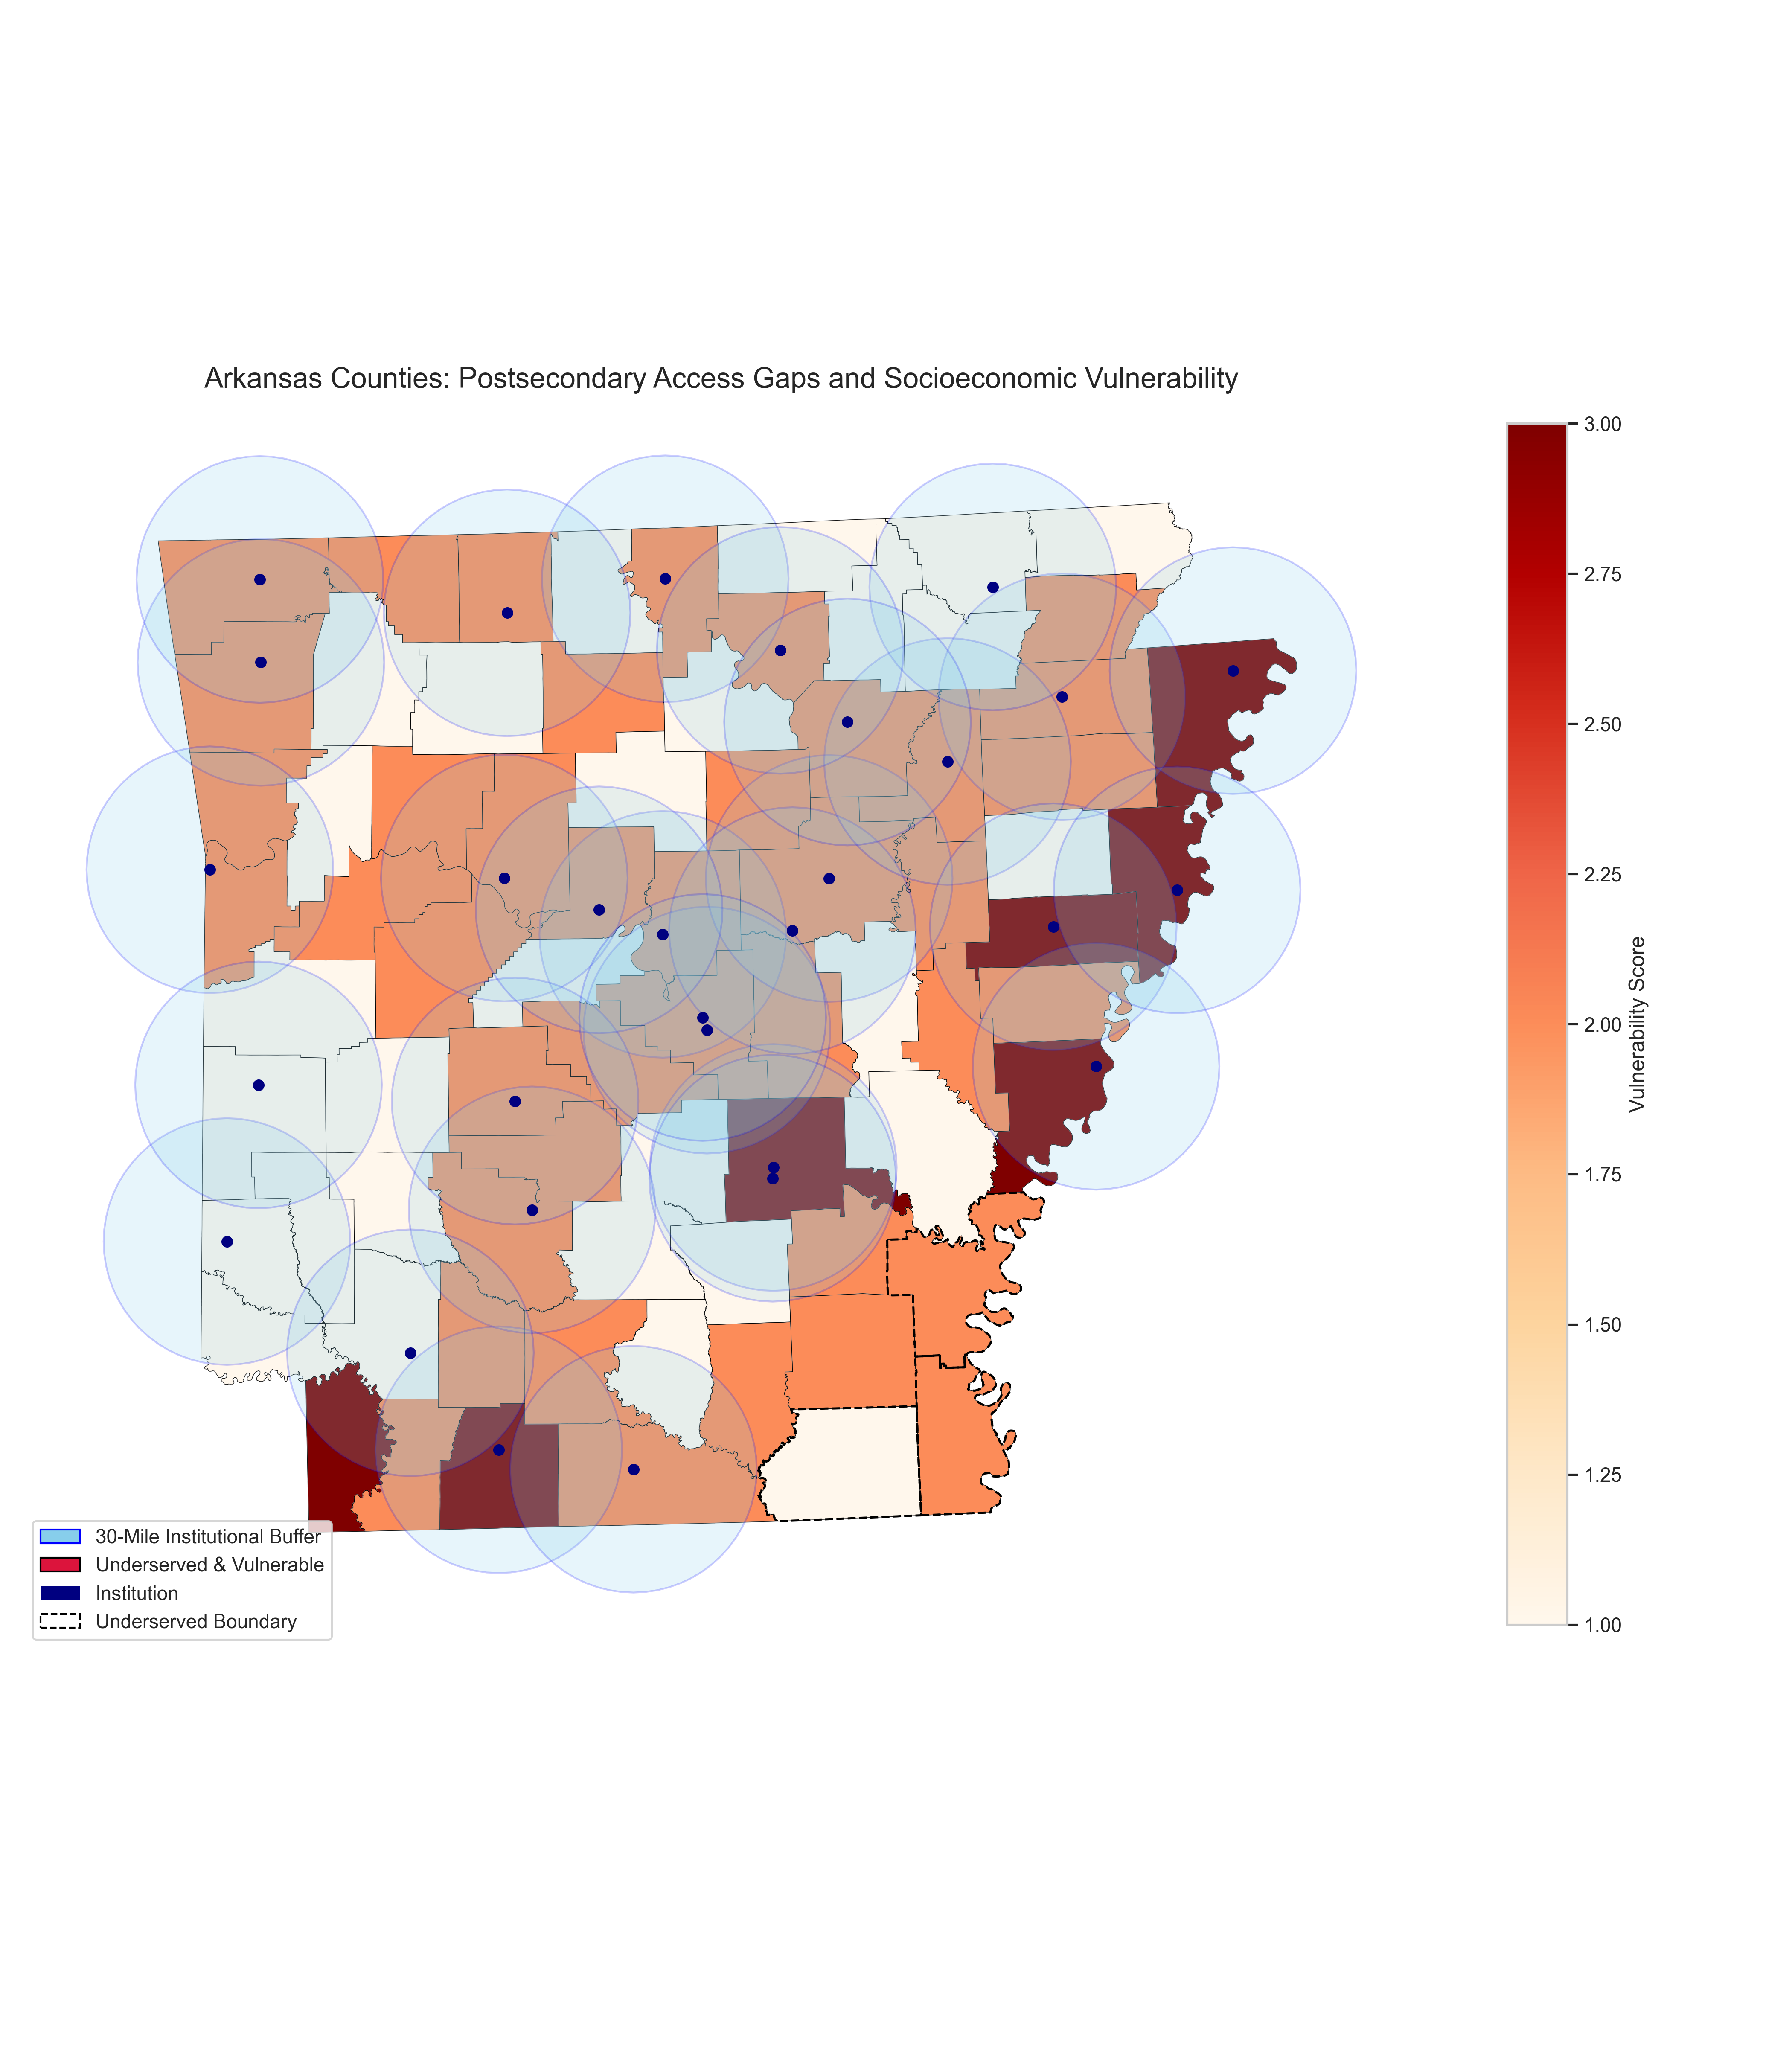
\includegraphics[width=0.95\textwidth]{images/maps/advanced_access_vulnerability_overlay_map.png}
\caption{Arkansas Counties: Postsecondary Access Gaps and Socioeconomic Vulnerability. The map overlays institutional access zones (30-mile buffers), population density, and county-level vulnerability scores. Crimson-shaded counties are outside institutional coverage and exhibit high composite vulnerability.}
\label{fig:access_vulnerability_map}
\end{figure}
















\section{Appendices}
\begin{itemize}
  \item A. Data dictionary
  \item B. Code/model summaries
  \item C. County-level snapshots
  \item D. Methodological notes
  \item E. North Central Arkansas Counties
  
\end{itemize}




\printbibliography

\begin{table}[!ht]
\centering
\caption{North Central Arkansas (NCA) Counties Used for Regional Comparison}
\label{tab:nca_counties}
\begin{tabular}{ll}
\hline
\textbf{County Name} & \textbf{Region/Notes} \\
\hline
Baxter     & Core Ozark Highlands \\
Boone      & Adjacent to Missouri border \\
Fulton     & Rural, northeastern NCA \\
Izard      & Central to regional education hub \\
Marion     & Near Buffalo National River \\
Newton     & Sparsely populated, forested terrain \\
Searcy     & Small population, rural infrastructure \\
Sharp      & Highland and Cherokee Village area \\
Stone      & Cultural heritage center (e.g., Mountain View) \\
Van Buren  & Border of Ozark and River Valley \\
Cleburne   & Greers Ferry Lake region \\
Independence & Batesville area, economic anchor \\
Lawrence   & Northeastern fringe of NCA \\
\hline
\end{tabular}
\end{table}









\end{document}
